\documentclass[a4paper, oneside, 11pt]{scrartcl}

% Get the necessary packages for the document.
% Set to english language and utf8.
\usepackage[english]{babel}
\usepackage[utf8]{inputenc}

% Some packages for symbols we need within the tutorial.
\usepackage{dingbat}
\usepackage{marvosym}

% For the sourcecode.
\usepackage{listings}

% For the links etc.
\usepackage[pdfborder={0 0 0}]{hyperref}

% For the pdf-graphics.
\usepackage{graphicx}

% The steamroller tactics to fix figures and so on.
\usepackage{float}

% This is for tables which are to long to be shown on one page.
\usepackage{longtable}

% This package is for the directory tree structures
\usepackage{dirtree}

% We need this package for some color within the document.
\usepackage{color}

% This is the package for the margin-nodes.
\usepackage[color=white, bordercolor=white]{todonotes}

\usepackage{amsfonts}
\usepackage{setspace}
\usepackage{ae,aecompl}

\usepackage[automark]{scrpage2}

\usepackage[margin=0.5cm,indention=-3em,font={sf},labelfont={bf,sf},format=hang]{caption}
% Get the new commands we defined for this document.
% The name of Kieker, just for the case that the design of this should change.
\newcommand{\Kieker}{\textsf{Kieker}}

% The current version-string.
\newcommand{\version}{1.5-trunk}

% The single parts of Kieker and some files.
\newcommand{\KiekerMonitoringPart}{\textsf{Kieker.Monitoring}}
\newcommand{\KiekerAnalysisPart}{\textsf{Kieker.Analysis}}
\newcommand{\analysisJar}{kieker-analysis-\version.jar}
\newcommand{\monitoringJar}{kieker-monitoring-\version.jar}
\newcommand{\commonJar}{kieker-common-\version.jar}
\newcommand{\toolsJar}{kieker-tools-\version.jar}
\newcommand{\commonsLoggingJar}{commons-logging-1.1.1.jar}
\newcommand{\monitoringPropertiesFile}{kieker.monitoring.properties}
\newcommand{\analysisPropertiesFile}{kieker.analysis.properties}
\newcommand{\logFourJPropertiesFile}{log4j.properties}
\newcommand{\aopFile}{aop.xml}

% The complete url where to find Kieker.
\newcommand{\KiekerURL}{\url{http://sourceforge.net/projects/kieker/files}}

% This is how we call the kieker directory.
\newcommand{\KiekerDir}{kieker-\version{}}%{$<$KIEKER-DIR$>$}

% These commands are necessary to mark classes, methods and files within the document.
\newcommand{\class}[1]{\texttt{#1}}
\newcommand{\method}[1]{\textit{#1}}
\newcommand{\dir}[1]{\texttt{#1}}
\newcommand{\file}[1]{\texttt{#1}}

% TODO command for our document
\newcommand{\TODO}[1]{\todo[inline,color=green!40]{TODO: #1}}

% These commands are for notifying the reader about something important.
\newcommand{\marginbox}[1]{\todo[noline]{#1}}
\newcommand{\notify}{\marginbox{\huge{\rightpointleft}}}
\newcommand{\warning}{\marginbox{\huge{\Stopsign}}}


% The following commands set the listings for the different (programming) languages correctly.
% For the first they use all nearly the same settings.
\newcommand{\setListing}[4]{
\lstset{
language=#1,          
numbers=#2,
basicstyle=#3,       	% the size of the fonts that are used for the code
showspaces=false,               % show spaces adding particular underscores
showstringspaces=false,         % underline spaces within strings
showtabs=false,                 % show tabs within strings adding particular underscores
%frame=shadowbox,	                % adds a frame around the code
frame=lrtb,
rulesepcolor=\color{black},
tabsize=2,	                % sets default tabsize to 2 spaces
captionpos=t,                   % sets the caption-position to bottom
breaklines=true,                % sets automatic line breaking
breakatwhitespace=false,        % sets if automatic breaks should only happen at whitespace
title=\lstname,                 % show the filename of files included with \lstinputlisting; also try caption instead of title
escapechar={#4}
}
}
\newcommand{\setJavaCodeListing}{\setListing{Java}{left}{\sffamily\scriptsize}{}}
\newcommand{\setBashListing}{\setListing{Bash}{none}{\sffamily\scriptsize}{°}}
\newcommand{\setXMLListing}{\setListing{XML}{none}{\sffamily\scriptsize}{}}


% Set the title and everything.
\title{Tutorial for \Kieker:\\ Monitoring and Analysis of Software Behavior}

% Here we go.
\begin{document}
  % We want a table of contents seperated from the rest of the text.
  \maketitle
  \tableofcontents
  \newpage

  \section{Overview}
    \subsection{What is \Kieker?}
      \Kieker\ is a framework\footnote{A framework is sort of a library or code fragment which provides specific and extended functionality.} which allows both programmers and software engineers the monitoring and analysis of program flows and the runtime behavior of java applications. Normal (``plain'') java applications can be arranged with the framework as well as server based java web applications. The framework itself aims to provide an easy managable and maintanable piece of software, which can be included uncomplicated into existing software projects. While \Kieker\ analyzes the own sourcecode reliably, it causes itself only very less overhead during monitoring. \Kieker\ can thereto put whole method calls on a watch, but single statements (e.g. a = a + 1) as well.\\
      Nearly every component of the framework can be extended and adjusted easily to the very own necessities.
      % This is the diagram which shows the single parts of Kieker as one component diagram (the 'satellite').
      \begin{figure}[H]
	\begin{center}
	  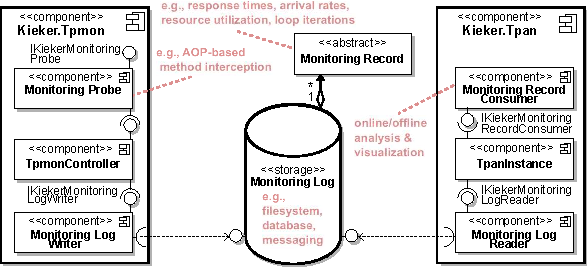
\includegraphics[width=1.0\textwidth]{kiekerComponentDiagram.pdf}
	  \label{image:kiekercomponentdiagram}
	  \caption{The component diagram of \Kieker}
	\end{center}
      \end{figure}
      As can be seen in figure \ref{image:kiekercomponentdiagram}, the framework consists mainly of two big parts:
      \begin{itemize}
	\item \textbf{\KiekerMonitoring}\\
	  This is the part which is responsible for the logging and the recording of the program behavior. The result of this component are the recorded informations which can then be written into different output streams, like for example into files or into a database.
	\item \textbf{\KiekerAnalysis}\\
	  This part is responsible for the evaluation and visualization of the recorded information. It uses the files (or general any collected data which is available as monitoring records) for the analysis and to produce graphs (e.g. Component-Dependency-Graph).
      \end{itemize}
      Both parts are composed each of three subcomponents which can be used or extended as well with own classes. The rough interaction between the different components is described by the following figure but will be explained furthermore in the course of this tutorial.
      % This is the diagram which shows the interaction between the components and when which component get what kind of input.
      \begin{figure}[H]
	\begin{center}
	  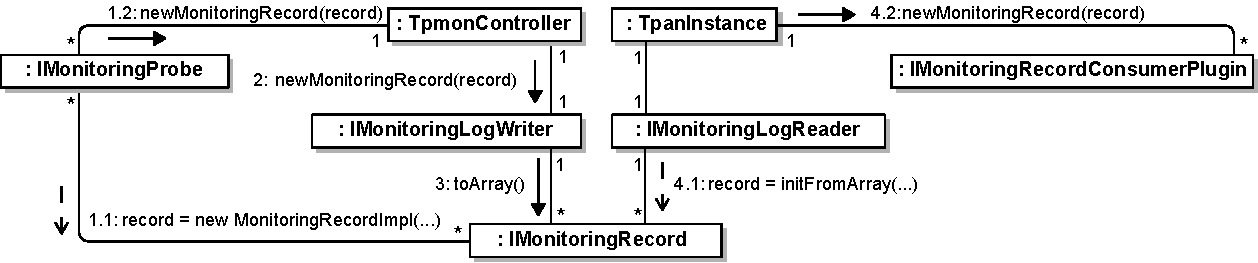
\includegraphics[width=1.0\textwidth]{kiekerCommunications-revisedReArranged-woMonitoringLog-bw.pdf}
	  \caption{Interaction between the components of \Kieker}
	\end{center}
      \end{figure}
      The monitoring probes create either the monitoring records manually or by calling the monitoring controller. The monitoring controller uses the monitoring log writers to persist the given records which can then be later read by a monitoring log reader who creates a monitoring record again. This monitoring recors can then be used by the consumer in nearly every way.

    \subsection{What ist the purpose of this tutorial?}
      In this tutorial, we will take a closer look at both, the \textbf{\KiekerMonitoring}- and the \textbf{\KiekerAnalysis}-part. That means, we will describe on the one hand how \KiekerMonitoring\ can be used to mark parts of the own sourcecode for \Kieker\ and to let them execute under surveilance, so that the recorded information can be saved somewhere and on the other hand we will use \KiekerAnalysis\ to process (for example visualize) our recorded data.\\
      We will show how to create and execute a simple example before we go deeper into the single parts of the framework.

  \section{Quickstart}
    \subsection{Downloading and installing \Kieker}
      For the monitoring and analysis of the source code, it is necessary to download the \Kieker\ binaries from \KiekerDownloadUrl\ first. Once that is done, the content of the zip- respectively the tar.gz-file should be extracted to any directory, for example ``$\sim$/kieker'' (under Linux) or ``c:$\backslash$program files$\backslash$kieker'' (under Windows).\\
      That is already enough for the ``installation'' of \Kieker. If desired, the new created path can of course be assigned to an easy remindable environment variable 
      % Note: Maybe it should be described how to do this.

    \subsection{Monitoring}
      Now for the creation of a simple example for the use of the \Kieker\ framework (note: The example is available on the website of \Kieker). It is recommended to create a new working directory (e.g. $\sim$/example) with the following subdirectories:
      \begin{itemize}
	\item src (For the sourcecode files)
	\item lib (For the libraries and needed jar-files)
	\item META-INF (For the configuration files of \Kieker)
	\item build (For the builded class files of Java)
      \end{itemize}
      Before we start with the source code, we need to copy some files from the \Kieker\ directory to our own working directory\footnote{It would be possible to access the required files within the \Kieker\ directory, but the copying will make the compiling much more comfortable.}.
      \begin{itemize}
	\item $\sim$/kieker/dist/\monitoringCtrlJar\ to $\sim$/example/lib/\monitoringCtrlJar
	\item $\sim$/kieker/lib/commons-logging-1.1.1.jar to $\sim$/example/lib/commons-logging-1.1.1.jar
        % Note: Is the log4j.properties really necessary? Seems to work without it.
	\item $\sim$/kieker/META-INF/log4j.properties.example to $\sim$/META-INF/\textbf{log4j.properties}
      \end{itemize}
      The last file is a configuration file, but for a quick start it is already configurated correctly.\\

      We start with creating two directories for our packages:
      % Note: This wouldn't be really necessary, but the package belonging is better visible.
      \begin{itemize}
	\item $\sim$/example/src/mySimpleKiekerExample
	\item $\sim$/example/src/mySimpleKiekerExample/bookstoreTracing
      \end{itemize}
      In the last directory, we create three files: 
      \begin{itemize}
	\item CRM.java
	\item Catalog.java
	\item Bookstore.java
      \end{itemize}
      The file ``Bookstore.java'' should contain of the lines showed in listing \ref{listing:Bookstore.java}.
      % It isn't necessary to do this every time but it makes sure that the listing has the correct format.
      \setJavaCodeListing
      % This will give the code a caption and - more important - a label which we can refer to.
      \lstset{caption=Bookstore.java, label=listing:Bookstore.java}
      % Careful! We load the file directly from the source directory. 
      \lstinputlisting{source-example/manual-monitoring/src/mySimpleKiekerExample/bookstoreTracing/Bookstore.java}
      Listing \ref{listing:Catalog.java} shows the content of ``Catalog.java'' and listing \ref{listing:CRM.java} the content of ``CRM.java''.
      \lstset{caption=Catalog.java, label=listing:Catalog.java}
      \lstinputlisting{source-example/manual-monitoring/src/mySimpleKiekerExample/bookstoreTracing/Catalog.java}
      \lstset{caption=CRM.java, label=listing:CRM.java}
      \lstinputlisting{source-example/manual-monitoring/src/mySimpleKiekerExample/bookstoreTracing/CRM.java}
      The monitoring itself is done manually. Although this is not the strength of \Kieker\ it is pretty good for a quick start.
      % It would be a waste of time to extract the part from the source-file. we do it manually.
      \lstset{caption=Cutting from Bookstore.java, label=listing:cuttingBookstore}
      \begin{lstlisting}
	long tin = TpmonController.getInstance().getTime();
	Bookstore.searchBook();
	long tout = TpmonController.getInstance().getTime();

	KiekerExecutionRecord e = KiekerExecutionRecord.getInstance("mySimpleKiekerExample.bookstoreTracing.Bookstore", "searchBook()", "sessionID", 0, tin, tout, "vnName", 0, 0);
	TpmonController.getInstance().logMonitoringRecord(e);
      \end{lstlisting}
      In listing \ref{listing:cuttingBookstore} can be seen, how the monitoring itself is done. We use the \textit{TpmonController} to get the current time in nano seconds and remember the time before and after a specific method call (in this case: \textit{searchBook()})\footnote{The code between the timekeeping does not need to be a method call of course. It can be ``plain'' code or more than one method call as well.}. These informations are stored in the so called execution record. It gets:
      % I am afraid it's a little bit complicate with the eoi and ess.
      \begin{itemize}
	\item The component (the class) in which the called method is.
	\item The called method.
	\item The session id. In this case we can use any string.
	\item The trace id of the current trace we want to record. Due to the fact, that we follow only one trace, this is zero in all recordings.
	\item The time before the sourcecode which should be measured.
	\item The time after the sourcecode which should be measured.
	\item The name of the current host. This is not very important in this case, because we have only one host. The name can be choosen freely.
	\item The eoi (execution order index). This tells \Kieker\ later the sequence of the different calls. It should be of course unique within a trace.
	\item The ess (execution stack size). This number tells \Kieker\ that the execution was started when the calling stack of the corresponding trace was just the                
              ess.
      \end{itemize}
      For the moment we have to choose the eoi and ess manually. These numbers can be choosen later automaticaly by \Kieker\ of course.\\
      Once the writing is done, we should be able to compile and execute the sourcecode:
      % We need something like the ouput from the bash.
      \setBashListing
      % Note: A little bit long...and the name of the libaries have to be changed manually.
      \begin{lstlisting}
	nils@Laptop:~/example$ javac ./src/mySimpleKiekerExample/bookstoreTracing/Bookstore.java ./src/mySimpleKiekerExample/bookstoreTracing/Catalog.java ./src/mySimpleKiekerExample/bookstoreTracing/CRM.java -classpath ./lib/kieker-monitoring-1.1-refactoring-branch_ctrl.jar:./lib/commons-logging-1.1.1.jar -d build/
	nils@Laptop:~/example$ java -Dlog4j.configuration=META-INF/log4j.properties -classpath ./build/:./lib/kieker-monitoring-1.1-refactoring-branch_ctrl.jar:./lib/commons-logging-1.1.1.jar mySimpleKiekerExample.bookstoreTracing.Bookstore
      \end{lstlisting}
      If everything worked correctly, there should now be a new directory named ``tpmon-20100605-115948636-UTC'' (just with other numbers) in the default temporary directory (under Linux this should be ``/tmp''). In this directory, there should be a file with the extension ``.dat'' with a content similar to the following:
      % Note: We don't have a suitable listing for 'plain' text. We use the bash listing for the moment.
      \begin{lstlisting}
	$1;1275745883934593403;-1;mySimpleKiekerExample.bookstoreTracing.Catalog.getBook(false);sessionID;0;1275745883931011663;1275745883933424540;vnName;1;1
	$1;1275745883937096236;-1;mySimpleKiekerExample.bookstoreTracing.Catalog.getBook(false);sessionID;0;1275745883935003302;1275745883937075214;vnName;3;2
	$1;1275745883937119354;-1;mySimpleKiekerExample.bookstoreTracing.CRM.getOffers();sessionID;0;1275745883934661568;1275745883937111043;vnName;2;1
	$1;1275745883937128922;-1;mySimpleKiekerExample.bookstoreTracing.Bookstore.searchBook();sessionID;0;1275745883931007961;1275745883937123824;vnName;0;0 
      \end{lstlisting}
      These are the recorded informations from our source code. This data can now be visualized with the help of \Kieker.

    \subsection{Analysis}
      % Here we go...we have to inform the user of the programs he need for the converting. And that means as well, that a window user cannot to this part.
      Assume that we already have our recorded informations saved in a ``.dat''-file somewhere for example in the ``tmp``-directory, we can now start with converting these informations into graphs. For the first, we change into our \Kieker\-directory ($\sim$/kieker). It is necessary to create a new directory for the graphs first:
\begin{lstlisting}
nils@Laptop:~/kieker$ mkdir /tmp/graphs
\end{lstlisting}
The shell-script ''./bin/trace-analysis.sh`` will now do most of the job.
\begin{lstlisting}
nils@Laptop:~/kieker$ ./bin/trace-analysis.sh --plot-Sequence-Diagrams --short-labels -i /tmp/tpmon-20100606-112536844-UTC/ -o /tmp/graphs/
\end{lstlisting}
The command ''--plot-Sequence-Diagrams`` tells the shell script to convert our data into a sequence diagram (other diagrams and graphs can be plot of course as well); with ''--short-labels`` we make sure that the components get a shorter name and the directories after ''-i`` and ''-o`` are the input- and the output-directories. If everything went well, \Kieker\ converted the data into files, which can now converted directly into visual graphs:
\begin{lstlisting}
nils@Laptop:~/kieker$ ./bin/dotPic-fileConverter.sh /tmp/graphs/ svg
\end{lstlisting}
The shell script ''./bin/dotPic-fileConverter.sh`` gets the directory with the files and the desired file extension (e.g. svg or png). The resulting graphs should now be available in ''/tmp/graphs`` and should look like the following:
\begin{figure}[H]
  \begin{center}
    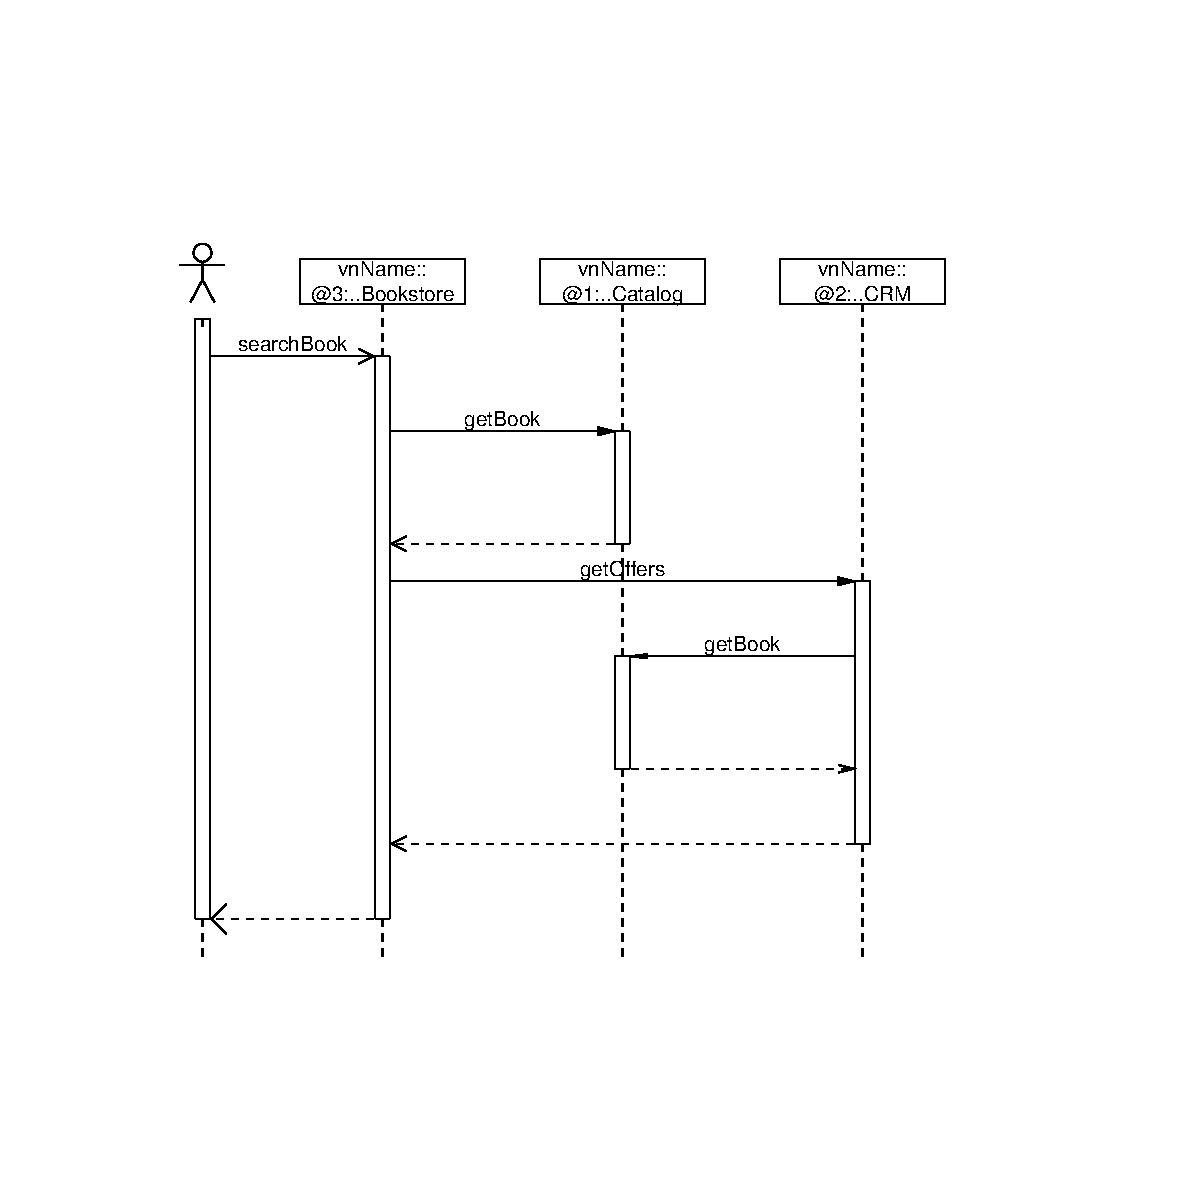
\includegraphics[width=0.5\textwidth]{sequenceDiagram.pdf}
    \label{image:sequencediagram}
    \caption{The resulting sequence diagram}
  \end{center}
\end{figure}
We are now able to monitor sourcecode in a simple way and to visualize these recorded informations.

\subsection{Using annotations}
Now we want to monitor whole methods without surrounding the method calls with a block where we keep the time manually. We will now use so called annotations to mark the methods we want to monitor. As can be seen in the following listing we write the annotation \textit{kieker.tpmon.annotation.TpmonExecutionMonitoringProbe} above the methods to be monitored. 
\setJavaCodeListing
\lstset{caption=Bookstore.java, label=listing:Bookstore2.java}
\lstinputlisting{source-example/annotation-monitoring/src/mySimpleKiekerExample/bookstoreTracing/Bookstore.java}
To make sure that the sourcecode is monitored, we need now aspectJ. Therefore we copy the file ''META-INF/aop.xml.example`` from our \Kieker\ directory to our working directory to ''META-INF/aop.xml``. In this file it is written which parts of the sourcecode will be monitored.  And we need another libarary as well. We copy $\sim$/kieker/dist/kieker-tpmon-\version\_ctw.jar to $\sim$/example/lib/kieker-tpmon-\version\_ctw.jar\\
To make sure that every method in our program which is annotated will be monitored, we have to write the following into the file:
\setXMLListing 
\begin{lstlisting}
<aspectj>
	<!-- turn verbose on to check which files are instrumented -->
	<!-- <weaver options="-verbose"/> -->
	<weaver options="">
	
	<!-- The following line is the important one -->
	<include within="*"/> 

	<!-- uncomment following to instrument sun jpetstore -->
\end{lstlisting}
The compiling is pretty much the same as before, but in order to run the program, we have to copy the configuration files into the build-directory.
\begin{lstlisting}
nils@Laptop:~/example$ javac ./src/Bookstore.java ./src/Catalog.java ./src/CRM.java -classpath ./lib/kieker-tpmon-1.1_ctrl.jar -d ./build
nils@Laptop:~/example$ cp -r ./META-INF/ ./build/META-INF
nils@Laptop:~/example$ java -Dlog4j.configuration=META-INF/log4j.properties -Dtpmon.configuration=META-INF/tpmon.properties -javaagent:lib/aspectjweaver-1.6.6.jar -Dorg.aspectj.weaver.showWeaveInfo=true -Daj.weaving.verbose=true -classpath ./build/:./lib/kieker-tpmon-1.1_ctrl.jar:./lib/kieker-common-1.1.jar:./lib/commons-logging-1.1.1.jar mySimpleKiekerExample.bookstoreTracing.Bookstore
\end{lstlisting}


\section{\KiekerMonitoring}
\subsection{Configuration}
The configuration possibilties of \KiekerMonitoring can be done in the configuration file named ''\monitoringPropertiesFile``. It is possible to activate/deactivate the monitoring and the debugging, set the target of the recorded informations or the path for the temporary paths of \Kieker. Most of the variables are self-explanatory.  
\subsection{Probes}
The probes (figure \ref{image:componentdiagram} shows them as well) decide which (and where) information should be recorded. To create own probes can for example be necessary if we want to record only specific data, or only every second method call and so on.
\subsection{Writers}
\hypertarget{monitoringlogwriters}
The so called \textit{monitoring log writers} (they can be seen as well in figure \ref{image:componentdiagram}) are the parts of \Kieker\ which are responsible for writing and serializing the recorded informations into files, databases and so on. In other words: They get an instance of \textit{AbstractKiekerMonitoringRecord} and produce an output of any nature whatsoever.\\
As can be seen in figure \ref{image:writers} there are already some writers implemented.
\begin{figure}[H]
	\begin{center}
		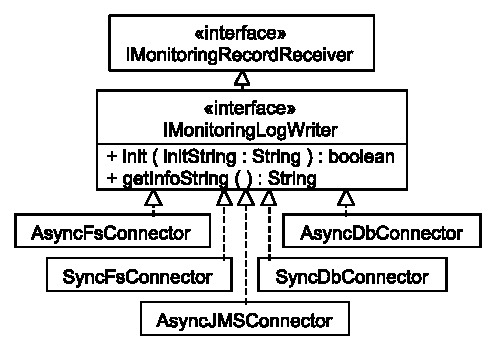
\includegraphics[width=0.5\textwidth]{kieker_writerimpls.pdf}
		\label{image:writers}
		\caption{The inheritance hierarchy of the current implemented monitoring log writers}
	\end{center}
\end{figure}
As the quick start part already showed it, every monitored record is sent to the \textit{TpmonController} which itself calls the current writer. The writer uses for example the \textit{toArray()} method of the record to get the informations stored by the record as handable array. The writer is then able to write these objects for example into a file. The used writer can be changed in the configuration file of \KiekerMonitoring.\\
To implement an own writer class, the following steps has to be performed:
\begin{enumerate}
 \item The new writer has to implement \textit{kieker.tpmon.writer.IMonitoringLogWriter}.
 \item All methods from the interfaces \textit{kieker.tpmon.writer.IMonitoringLogWriter} and \textit{kieker.common.record.IMonitoringRecordReceiver} has to be implemented.
 \item The entry \textit{monitoringDataWriter} has to be changed in the configuration file ''tpmon.properties`` to the entire classname.
\end{enumerate}
The following example writer takes the informations from the given record and shows them just on the screen.
\setJavaCodeListing
%\lstset{caption=OwnWriter.java, label=listing:OwnWriter.java}
%\lstinputlisting{source-example/manual-monitoring-with-own-writer/src/mySimpleKiekerExample/bookstoreTracing/MyWriter.java}

\section{\KiekerAnalysis}
The part of \Kieker\ which is responsible for the analysis consist of the reader, the consumer and the analysis instance itself. After we stored somewhere our records, we need to read them again somehow. This is task of the reader. Whatever we want to do with these informations is task of the consumers. They can for example evaluate, process or visualize the data. The analysis instance concerns about the lifetime and registration of the other parts.\\
The analysis consists roughly of the following steps:
\begin{enumerate}
 \item Create one (or more) analysis instance.
 \item Set the reader of this instance and line it with the necessary informations to read the stored records.
 \item Register the consumers who should do something with the recorded data.
 \item Start the analysis instance.
\end{enumerate}
\subsection{Configuration}
The configuration of \KiekerAnalysis\ will later be possible in the file ''\analysisPropertiesFile``. At the moment it is not necessary to set any properties due to the fact, that we concern about the analysis ourselves. 
\subsection{Readers}
\begin{figure}[H]
	\begin{center}
		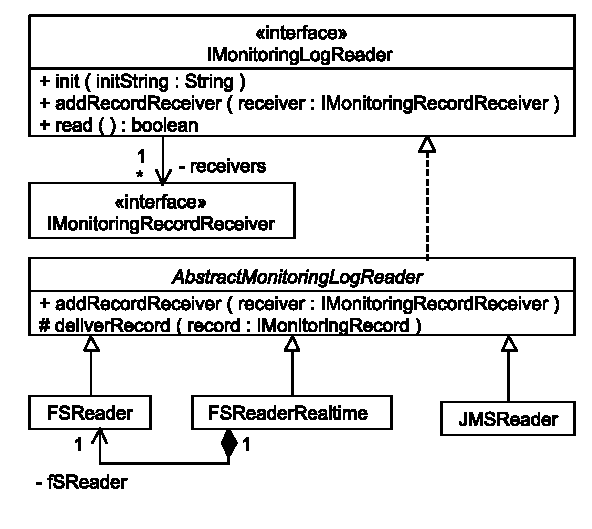
\includegraphics[width=0.5\textwidth]{kieker_readerimpls.pdf}
		\label{image:readers}
		\caption{}
	\end{center}
\end{figure}
The \textit{monitoring log readers} (their position can be found in figure \ref{image:componentdiagram}) are the counterpart to the \hyperlink{monitoringlogwriters}{\textit{monitoring log writers}}. While the writers get a record and write them in files or somewhere else, the readers take the writen data (from files, databases and so on) and convert them into an \textit{AbstractKiekerMonitoringRecord}. That means, that whenever we are implementing a new writer, we should also implement a corresponding reader. If we want for example save our recorded informations in a database, we have to be capable of reading these stored informations from the database again. The implementing of an own reader is nearly the same as the implementing of the writer, but to keep things simple, it is recommended to extend the already implemented AbstractKiekerMonitoringLogReader, because otherwise it would be necessary to implement the used observer pattern of the reader. 
\begin{enumerate}
 \item The new reader has to extend \textit{kieker.common.logReader.AbstractKiekerMonitoringLogReader}.
 \item All methods from the interface  \textit{kieker.common.logReader.IKiekerMonitoringLogReader} which has not been implemented yet by the class must be implemented.
\end{enumerate}

\subsection{Consumers}
The consumer is the part of \Kieker\ which decides what to do with the stored informations. 
\section{Appendix}
\subsection{Example logs}
\subsection{Shortcut via ant}
\subsection{Libraries}
\begin{center}
\begin{longtable}{|p{0.4\textwidth}|p{0.5\textwidth}|}
\hline 
Filename & Description\\
\hline
\hline 
commons-cli-1.2.jar & n/a\\
\hline 
maven & n/a\\
\hline 
mysql-connector-java-5.1.5-bin.jar & The library to connect to an existing MySQL database.\\
\hline 
spring-web.jar & n/a\\
\hline 
Scenario.jar & n/a\\
\hline 
sequence.pic & n/a\\
\hline 
openjms-0.7.7-beta-1.tar.gz & n/a\\
\hline 
aspectjrt-1.6.6.jar & n/a\\
\hline 
commons-logging-1.1.1.jar & n/a\\
\hline 
aspectjtools-1.6.6.jar & n/a\\
\hline 
jms-1.1.jar & n/a\\
\hline 
concurrent-1.3.4.jar & n/a\\
\hline 
servlet.jar & n/a\\
\hline 
pmd & n/a\\
\hline 
spring.jar & n/a\\
\hline 
openjms-common-0.7.7-beta-1.jar & n/a\\
\hline 
servlet-api.jar & n/a\\
\hline 
commons-pool-1.2.jar & n/a\\
\hline 
derby.jar & This library contains the necessary drivers for the Apache Derby database.\\
\hline 
commons-io-1.2.jar & n/a\\
\hline 
cxf-rt-core-2.2.6.jar & n/a\\
\hline 
jmc.jar & n/a\\
\hline 
log4j-1.2.15.jar & n/a\\
\hline 
openjms-net-0.7.7-beta-1.jar & n/a\\
\hline 
aspectjweaver-1.6.6.jar & n/a\\
\hline 
cxf-api-2.2.6.jar & n/a\\
\hline 
rabbitmq-client.jar & n/a\\
\hline 
openjms-0.7.7-beta-1.jar & n/a\\
\hline 
spice-jndikit-1.2.jar & n/a\\
\hline 
cxf-rt-bindings-soap-2.2.6.jar & n/a\\
\hline 
cxf-common-utilities-2.2.6.jar & n/a\\
\hline 
jndi-1.2.1.jar & n/a\\
\hline 
\end{longtable}
\label{tabular:libraries}
\end{center}

\subsection{Troubleshooting}
\end{document}
 
